%% REPLACE sXXXXXXX with your student number
\def\studentNumber{s2187249}


%% START of YOUR ANSWERS
%% Add answers to the questions below, by replacing the text inside the brackets {} for \youranswer{ "Text to be replaced with your answer." }. 
%
% Do not delete the commands for adding figures and tables. Instead fill in the missing values with your experiment results, and replace the images with your own respective figures.
%
% You can generally delete the placeholder text, such as for example the text "Question Figure 2 - Replace the images ..." 
%
% There are 19 TEXT QUESTIONS (a few of the short first ones have their answers added to both the Introduction and the Abstract). Replace the text inside the brackets of the command \youranswer with your answer to the question.
%
% There are also 3 "questions" to replace some placeholder FIGURES with your own, and 3 "questions" asking you to fill in the missing entries in the TABLES provided. 
%
% NOTE! that questions are ordered by the order of appearance of their answers in the text, and not by the order you should tackle them. Specifically, you cannot answer Questions 2, 3, and 4 before concluding all of the relevant experiments and analysis. Similarly, you should fill in the TABLES and FIGURES before discussing the results presented there. 
%
% NOTE! If for some reason you do not manage to produce results for some FIGURES and TABLES, then you can get partial marks by discussing your expectations of the results in the relevant TEXT QUESTIONS (for example Question 8 makes use of Table 1 and Figure 2).
%
% Please refer to the coursework specification for more details.

%% - - - - - - - - - - - - TEXT QUESTIONS - - - - - - - - - - - - 

%% Question 1:
\newcommand{\questionOne} {
\youranswer{a condition where the network function too closely fits to the training set and results in poor generalization}
}

%% Question 2:
\newcommand{\questionTwo} {
\youranswer{Question 2 - Summarise the effect increasing width and depth of the architecture had on overfitting}
\youranswer{Question 2 - can generally make the neural network more easily to be overfitting}
}

%% Question 3:
\newcommand{\questionThree} {
\youranswer{Question 3 - Summarise what your results show you about the effect of the tested approaches on overfitting and the performance of the trained model}
}

%% Question 4:
\newcommand{\questionFour} {
\youranswer{Question 4 - Give your overall conclusions}
}

%% Question 5:
\newcommand{\questionFive} {
\youranswer{it has a poor performance on the validation set or test set,
in sharp contrast to its' rather good performance on the training set. In short, it has poor ability for generalization}
}

%% Question 6:
\newcommand{\questionSix} {
\youranswer{Overfitting occurs when the model learns too much about and fits too close to the training set, and then lose the ability to generalize to the unseen data.
This could be identified based on the increasing validation error after some point and the inceasing gap between the performance on validation set and training set.}
}

%% Question 7:
\newcommand{\questionSeven} {
\youranswer{it is about the relationship between epoch and accuracy, containing 2 curves which represent accuracy on training set and test set respectively.
And for Figure 1b, it is about the relationship between epoch and error, containing 2 curves which represent accuracy on training set and test set respectively.
As is the same point in both figures, we can see that the difference on $\by$ value between training set and validation set generally increases along the epoch
number when epoch>10. For more details, you can see that the accuracy on validation set nearly reaches a maximum at epoch 10, and then decreases along the epoch, while the accuracy
on training set keeps increasing in the Figure 1a. The similar case also happens in Figure 1b, but the curves move in the opposite direction.
Based on the idea that overfitting shows as the increasing gap between performance on training set and validation set, we can simply infer that
the overfitting actually occur at nearly epoch 10 according to these Figures.
}
}

%% Question 8:
\newcommand{\questionEight} {
\youranswer{The generalization gap increases with the increasement of hidden units in the final epoch in contrast to the slight changes in validation accuracy,
 which indicts that the adding more hidden units may not improve the final performance but make the overfitting more serious in this case. From the Figure 2, we
 can also observe that actually the best result on validation set of network with width 64 and 128 already reaches at nearly epoch 10. However, after this point,
 their performance starts to drop along the epoch number and the generalization gap also increases. But for the network with width 32, we can see that its performance
 on the validation set actually becomes better along the epoch number.}
}

%% Question 9:
\newcommand{\questionNine} {
\youranswer{The width of the network could affect extent of overfitting in a nearly linear way. Generally speaking, adding more hidden units could make the network
more likely to be overfitting and make the overfitting more serious. However, in spite of the more serious overfitting conditions for width 64 and 128 in this case,
they finally get a slightly higher accuary than the width 32. So, could we say that a wider network will be a better choice in this case?
Based on the previous knowledge, the wider the network, the stronger fitting ability it will have, it would have a better result than narrow networks if the overfitting does not
happen. But it has a higher chance to get overfitting. This actually matches our experiment since the wider network (64 and 128) does better before overfitting (nearly at epoch 10) in this case.
However, their performance on validation set keeps droping after that. We could expect that its accuracy and error may even be much worse than that of width 32 if we make the epoch number larger.
So, for a wider network, we should carefully choose the epoch number to avoid overfitting, otherwise the overfitting will make the wider networks a bad choice.}
}

%% Question 10:
\newcommand{\questionTen} {
\youranswer{The curves are very close to the each other in the same category. That is, they have the nearly the same tendency and the similar value on the traing set or validation set
according to the same epoch number. In general, they all keep increasing their performance on the training set along epoch. However, in terms of their performance on the validation set,
they reach a maximum performance at nearly epoch 10, and then keep dropping along the epoch, which indicates the overfitting occurs. In short, we can not observe obvious change according
to the change of network depth.}
}

%% Question 11:
\newcommand{\questionEleven} {
\youranswer{According to the observed result, we actually could not draw conclusions about the network depth since all the curves shown in Figure 2 behave in a similar way.
The only difference we could get is that, the model with different depth could have slightly different error on the training set. But we acctually do not care their performance
on the training set. Based on the previous lecture, adding more hidden layers could have the similar effect as adding more hidden units, which is better fitting ability
but with the larger chance to get overfitting. However, this experiment does not prove our knowledge in this case because the varying layers do not bring obvious change in
The Figure 2. The possible reason for this may be that the width of 128 in the hidden layers could easily cause overfitting, making the effect of varying depth not so obvious
in this case. If we change the width of hidden layers to 32, we may spot the changes and draw conclusions more easily.}
}

%% Question 12:
\newcommand{\questionTwelve} {
\youranswer{From the expriments mentioned above, we can draw that adding width and adding depth can similar effect. That is, the model will have the better fitting ability, but
suffer more possibility to be overfitting. In addition, if the overfitting does not occur, wider and deeper neural networks could generally have a better performance
on the validation set than narrower and shallower networks before overfitting. However, after getting overfitting, they could even have a worse performance than the
the narrower and shallower ones. Based on the ideas listed above, we should carefully tune the width and depth of the networks, otherwise they could easily get overfitting when
the epoch number is large.}
}

%% Question 13:
\newcommand{\questionThirteen} {
\youranswer{L1 and L2 regularization mean that we will finally add a term related to the neural network weight $\bw$ when computing the lost function, with the intention of making
the network not so flexible by putting some constraints on $\bw$. In particular, the L1 regularization uses first power term to deal with $\bw$. It adds $\lambda_1\sum_w{\lvert \bw_i \rvert}$
to the lost function. The  L1 regularization uses quadratic term to deal with $\bw$. It adds $\lambda_2\sum_w \bw_i^2 \rvert$to the lost function. In the 2 formulas mentioned above, the
parameters $\lambda_1$ and $\lambda_2$ are the hyper-parameter we need to set by ourself according to specific training conditions. These terms mentioned
above will be counted into the final lost  function, which the neural network tries to minimize. In addition, these terms will also take in the part of computing gradients.}
}

%% Question 14:
\newcommand{\questionFourteen} {
\youranswer{Since the L1 regularization and L2 regularization methods both add a term related to the weight $\bw$, the neural network will try to minimize the new lost function
    (original lost function + regularization term). Since the regularization term involves weight $\bw$, the neural network then tend not to use the larger $\bw$ to fit the data
more flexible, but rather to use smaller $\bw$ to smoothly fit the data, resulting in a better generalization to the unseen data. Thus these regularizations can alleviate overfitting
to some extent. L1 regularization uses first power term, its gradients would be $\lambda_1 sign_{+-}(w_i)$ for the weight $\bw_i$, while $2\lambda_2w_i$ for L2 regularization.
As we can see in the two gradients, the L1 regularization punishes the weight $\bw_i$ in a constant way while the L2 regularization punishes the weight $\bw_i$ in relationship with $\bw_i$.
We can image that, after several epoches, the $\bw_i$  could become 0 under L1 regularization, but may not become 0 under L2 regularization beacause the gradients is related to  $\bw_i$ value.
As a result, L1 regularization may set some $\bw_i$ to 0, whose process could be viewed as feature selection by removing some useless $\bw_i$. It finally alleviates overfitting by removing some features.
L2 reularization tries to achieve a balance between the original lost function and L2 term. And finally it can also alleviate overfitting by making the fitting line smoother since these
$\bw_i$ will not be too deviated from 0 under L2 regularization.}
}

%% Question 15:
\newcommand{\questionFifteen} {
\youranswer{Question 15 - Explain the experimental details (e.g. hyperparameters), discuss the results in terms of their generalization performance and overfitting}
}

%% Question 16:
\newcommand{\questionSixteen} {
\youranswer{it has not previously been demonstrated to actually perform model averaging for deep architectures}
}

%% Question 17:
\newcommand{\questionSeventeen} {
\youranswer{The Dropout is compatible with Maxout. Based on the standard practice, \cite{goodfellow2013maxout} found that the combination of Maxout and Dropout can
make a more robust network and tend to achieve great performance. By principle, different dropout masks tend to put inputs far enough to escape the local region surrounding
the clean inputs where the hidden units are linear. Maxout trained with dropout may have  the identity of the maximal filter in each unit change relatively rarely as the dropout mask changes. Net-
works of linear operations and max(·) may learn to exploit dropout’s approximate model averaging technique well.}
}

%% Question 18:
\newcommand{\questionEighteen} {
\youranswer{Question 18 - Give an overview of the experiment setup in \cite{goodfellow2013maxout} and analyse it from the point of view of how convincing their conclusions are
}
}

%% Question 19:
\newcommand{\questionNineteen} {
\youranswer{Question 19 - Briefly draw your conclusions based on the results from the previous sections (what are the take-away messages?) and conclude your report with a recommendation for future directions
}
}


%% - - - - - - - - - - - - FIGURES - - - - - - - - - - - - 

%% Question Figure 2:
\newcommand{\questionFigureTwo} {
\youranswer{Question Figure 2 - Replace the images in Figure 2 with figures depicting the accuracy and error, training and validation curves for your experiments varying the number of hidden units.

\begin{figure}[t]
    \centering
    \begin{subfigure}{\linewidth}
        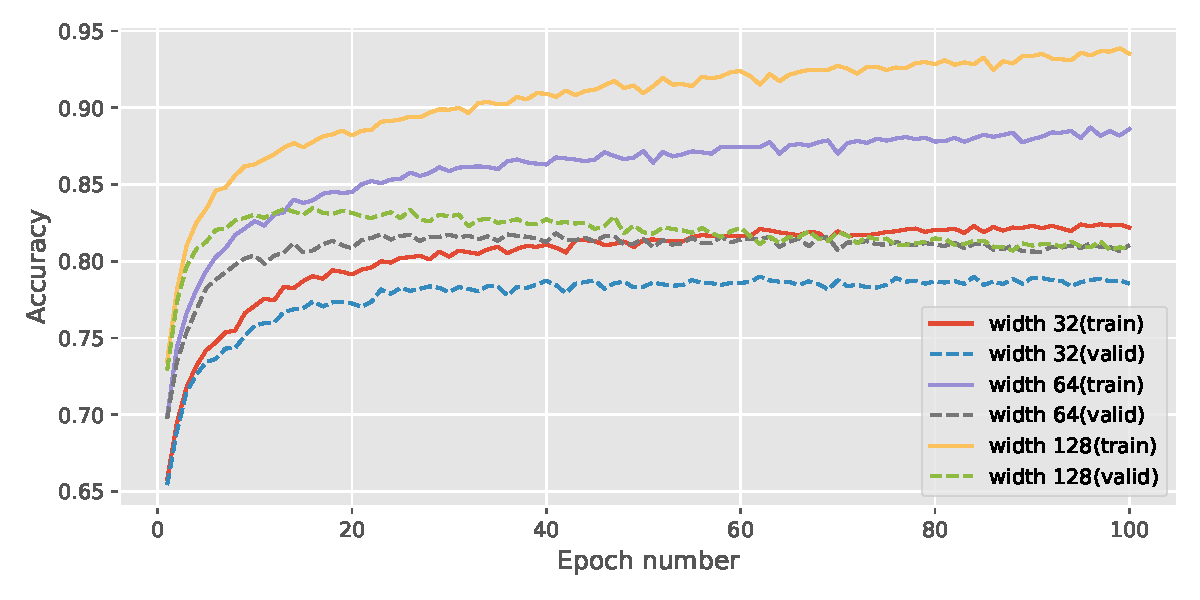
\includegraphics[width=\linewidth]{figures/acc_curve_width.pdf}
        \caption{accuracy by epoch}
        \label{fig:width_acccurves}
    \end{subfigure}
    \begin{subfigure}{\linewidth}
        \centering
        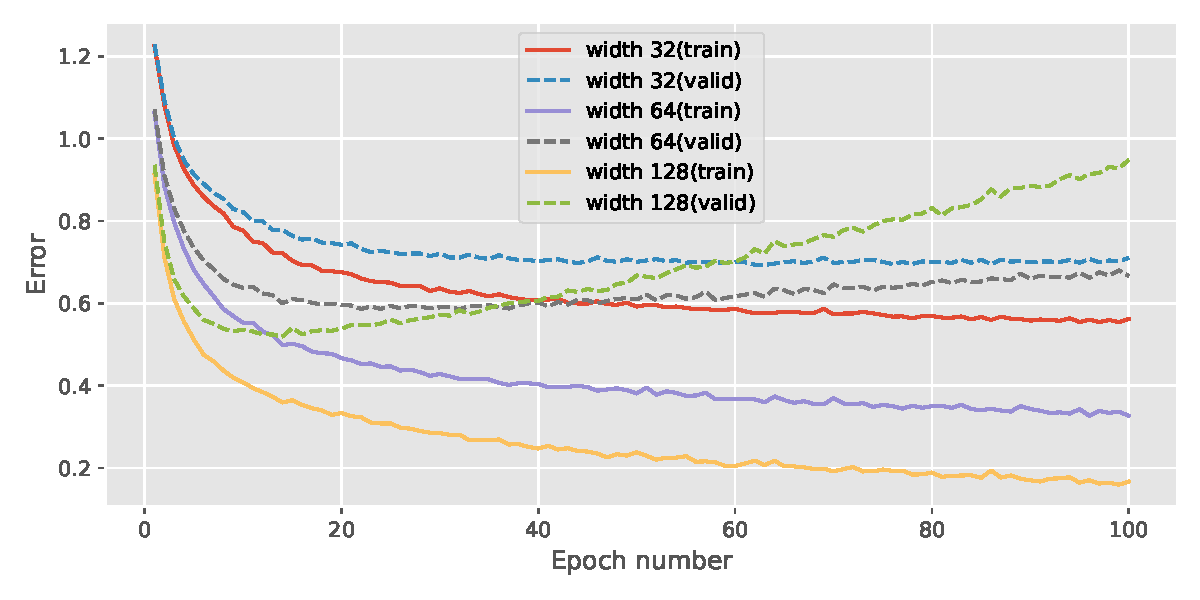
\includegraphics[width=\linewidth]{figures/error_curve_width.pdf}
        \caption{error by epoch}
        \label{fig:width_errorcurves}
    \end{subfigure}
    \caption{Training and validation curves in terms of classification accuracy (a) and cross-entropy error (b) on the EMNIST dataset for different network widths.}
    \label{fig:width}
\end{figure}

}
}

%% Question Figure 3:
\newcommand{\questionFigureThree} {
\youranswer{Question Figure 3 - Replace these images with figures depicting the accuracy and error, training and validation curves for your experiments varying the number of hidden layers.

\begin{figure}[t]
    \centering
    \begin{subfigure}{\linewidth}
        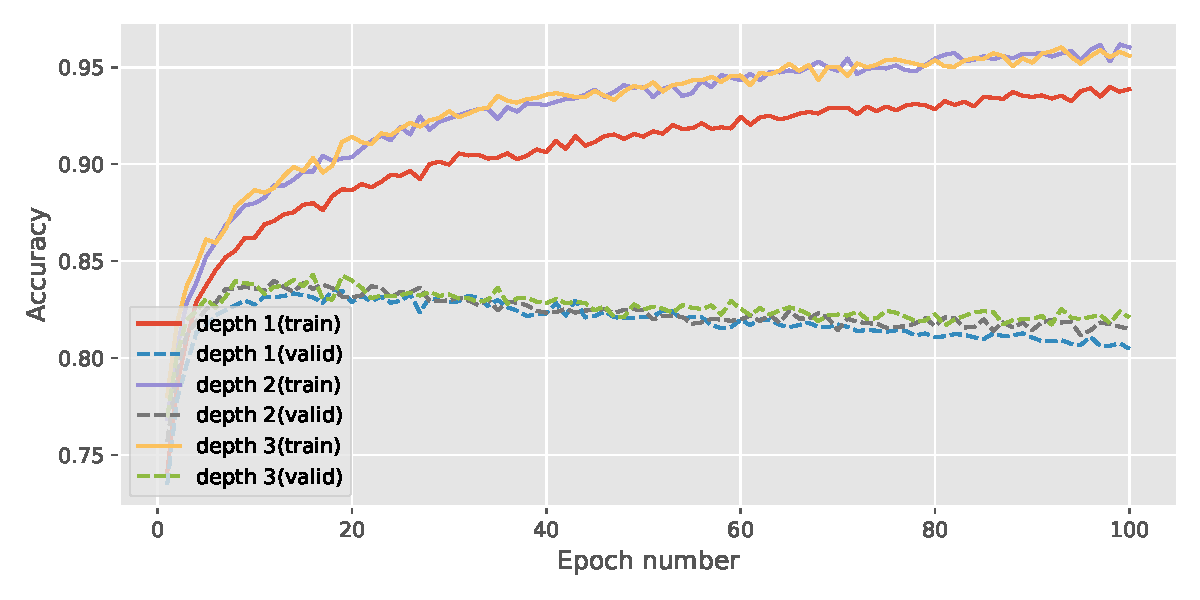
\includegraphics[width=\linewidth]{figures/acc_curve_depth.png}
        \caption{accuracy by epoch}
        \label{fig:depth_acccurves}
    \end{subfigure}
    \begin{subfigure}{\linewidth}
        \centering
        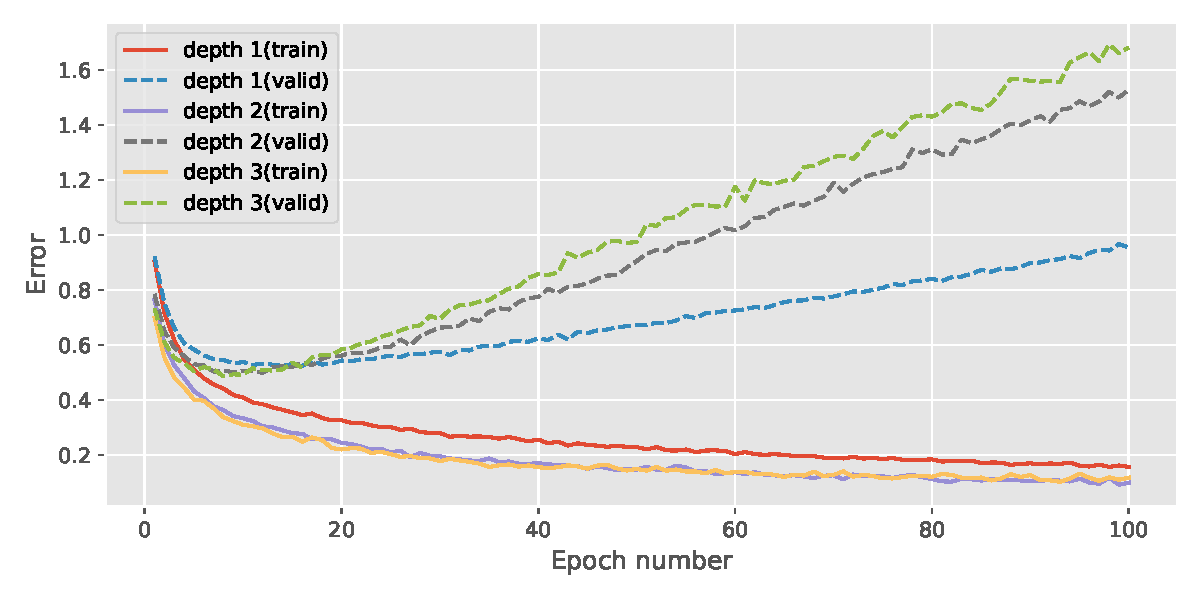
\includegraphics[width=\linewidth]{figures/error_curve_depth.png}
        \caption{error by epoch}
        \label{fig:depth_errorcurves}
    \end{subfigure}
    \caption{Training and validation curves in terms of classification accuracy (a) and cross-entropy error (b) on the EMNIST dataset for different network depths.}
    \label{fig:depth}
\end{figure}

}
}

%% Question Figure 4:
\newcommand{\questionFigureFour} {
\youranswer{Question Figure 4 - Replace these images with figures depicting the Validation Accuracy and Generalisation Gap for each of your experiments varying the Dropout rate, L1/L2 weight penalty, and for the 8 combined experiments (you will have to find a way to best display this information in one subfigure).

\begin{figure*}[t]
    \centering
    \begin{subfigure}{.3\linewidth}
        \includegraphics[width=\linewidth]{figures/empty_dropout_plot.png}
        \caption{Metrics by dropout rate}
        \label{fig:dropoutrates}
    \end{subfigure}
    \begin{subfigure}{.3\linewidth}
        \centering
        \includegraphics[width=\linewidth]{figures/empty_wd_plot.png}
        \caption{Metrics by weight penalty}
        \label{fig:weightrates}
    \end{subfigure}
    \begin{subfigure}{.3\linewidth}
        \centering
        \includegraphics[width=.85\linewidth]{example-image-duck}
        \caption{Extra experiments}
        \label{fig:extra}
    \end{subfigure}
    \caption{Hyperparameter search for every method and combinations}
    \label{fig:hp_search}
\end{figure*}

}
}

%% - - - - - - - - - - - - TABLES - - - - - - - - - - - - 

%% Question Table 1:
\newcommand{\questionTableOne} {
\youranswer{
Question Table 1 - Fill in Table 1 with the results from your experiments varying the number of hidden units.

\begin{table}[t]
    \centering
    \begin{tabular}{c|cc}
    \toprule
        \# hidden units & val. acc. & generalization gap \\
    \midrule
         32            &     79.73\%    &             0.18        \\
         64            &     80.70\%     &            0.53       \\
         128           &     81.67\%     &            1.44        \\
    \bottomrule
    \end{tabular}
    \caption{Validation accuracy (\%) and generalization gap (in terms of cross-entropy error) for varying network widths on the EMNIST dataset.}
    \label{tab:width_exp}
\end{table}
}
}

%% Question Table 2:
\newcommand{\questionTableTwo} {
\youranswer{
Question Table 2 - Fill in Table 2 with the results from your experiments varying the number of hidden layers.

\begin{table}[t]
    \centering
    \begin{tabular}{c|cc}
    \toprule
        \# hidden layers & val. acc. & generalization gap \\
    \midrule
         1               &      81.58\%      &       1.41             \\
         2               &      82.08\%      &        1.59            \\
         3               &      82.27\%      &        1.28           \\
    \bottomrule
    \end{tabular}
    \caption{Validation accuracy (\%) and generalization gap (in terms of cross-entropy error) for varying network depths on the EMNIST dataset.}
    \label{tab:depth_exps}
\end{table}
}
}

%% Question Table 3:
\newcommand{\questionTableThree} {
\youranswer{
Question Table 3 - Fill in Table 3 with the results from your experiments varying the hyperparameter values for each of L1 regularisation, L2 regularisation, and Dropout (use the values shown on the table) as well as the results for your experiments combining L1/L2 and Dropout (you will have to pick what combinations of hyperparameter values to test for the combined experiments; each of the combined experiments will need to use Dropout and either L1 or L2 regularisation; run an experiment for each of 8 different combinations). Use \textit{italics} to print the best result per criterion for each set of experiments, and \textbf{bold} for the overall best result per criterion.

\begin{table*}[t]
    \centering
    \begin{tabular}{c|c|cc}
    \toprule
        Model    &  Hyperparameter value(s) & Validation accuracy & Generalization gap \\
    \midrule
    \midrule
        Baseline &       lr=0.001, hidden layers = 3, hidden units = 128                &           82.5 \%           &        1.30           \\
    \midrule
        \multirow{5}*{Dropout}
                 & 0.1                   &           2.67\%          &          5.30e-3           \\
                 & 0.3                   &           52.81\%          &         0.03           \\
                 & 0.5                   &          76.08\%           &         0.07           \\
                 & 0.7                   &           83.15\%          &         0.11          \\
                 & 0.9                   &          85.52\%           &         0.24          \\
    \midrule
        \multirow{5}*{L1 penalty}
                 & 1e-5                   &         82.98\%            &        0.74           \\
                 & 1e-4                   &         85.36\%            &        0.10           \\
                 & 1e-3                   &         75.65\%            &        0.02          \\
                 & 1e-2                   &          1.96\%           &         4.46e-4          \\
                 & 1e-1                   &          2.01\%           &         4.87e-4          \\
    \midrule
        \multirow{5}*{L2 penalty}
                 & 1e-5                   &         82.68\%          &         1.09          \\
                 & 1e-4                   &         83.42\%            &       0.50            \\
                 & 1e-3                   &         85.09\%            &       0.08           \\
                 & 1e-2                   &         76.68\%           &        0.01           \\
                 & 1e-1                   &          1.98\%           &        4.4e-4           \\
    \midrule
        \multirow{8}*{Combined}
                 & for example 0.95, L1 1e-6  &                     &                   \\
                 & ?, ?                   &                     &                   \\
                 & ?, ?                   &                     &                   \\
                 & ?, ?                   &                     &                   \\
                 & ?, ?                   &                     &                   \\
                 & ?, ?                   &                     &                   \\
                 & ?, ?                   &                     &                   \\
                 & ?, ?                   &                     &                   \\
    \bottomrule
    \end{tabular}
    \caption{Results of all hyperparameter search experiments. \emph{italics} indicate the best results per series and \textbf{bold} indicate the best overall}
    \label{tab:hp_search}
\end{table*}

}
}

%% END of YOUR ANSWERS